% Copyright © 2016 Lukas Rosenthaler, Benjamin Geer, Ivan Subotic,
% Tobias Schweizer, André Kilchenmann, and André Fatton.
%
% This file is part of Knora.
%
% Knora is free software: you can redistribute it and/or modify
% it under the terms of the GNU Affero General Public License as published
% by the Free Software Foundation, either version 3 of the License, or
% (at your option) any later version.
%
% Knora is distributed in the hope that it will be useful,
% but WITHOUT ANY WARRANTY; without even the implied warranty of
% MERCHANTABILITY or FITNESS FOR A PARTICULAR PURPOSE.  See the
% GNU Affero General Public License for more details.
%
% You should have received a copy of the GNU Affero General Public
% License along with Knora.  If not, see <http://www.gnu.org/licenses/>.
%-----------------------------------------------------------------------%

% This file contents notes and wireframe samples for the web app interface of Knora: (called) SALSAH 2

\documentclass[12pt]{article} % Default font size is 12pt, it can be changed here
%-------------------------%
%   file configuration    %
%-------------------------%
\usepackage{cmap}
\usepackage[utf8]{inputenc}
\usepackage[ngerman, english]{babel}
\usepackage[T1]{fontenc}

\usepackage[dmyy]{datetime}
\renewcommand{\dateseparator}{.}

\usepackage{geometry} % Required to change the page size to A4
\geometry{a4paper} % Set the page size to be A4 as opposed to the default US Letter

\usepackage{graphicx} % Required for including pictures
\graphicspath{{images/}{images/mockups/}{images/inspiration/}} % Specifies the directory where pictures are stored
\usepackage[font=footnotesize]{caption} % smaller image description

\usepackage{float} % Allows putting an [H] in \begin{figure} to specify the exact location of the figure
\usepackage{wrapfig} % Allows in-line images such as the example fish picture

\usepackage{anysize} %Damit man Raender leicht einstellen kann
%\marginsize{3cm}{3cm}{2cm}{2.0cm} %Raender

\usepackage{setspace} %Zeilenabstand
\linespread{1.5} % Line spacing
%\onehalfspacing % One half line spacing

\setlength{\parindent}{0pt} % damit wird die erste Zeile nicht eingerückt!

\newcommand{\HRule}{\rule{\linewidth}{0.2mm}} % Defines a new command for the horizontal lines, change thickness here

\usepackage{fancyheadings} % Header and Footer
% 1. clear de default layout
\fancyhead{}
\fancyfoot{}
% 2. create your own header and footer style in your document


% setting for widows and orphans
\widowpenalty=10000
\clubpenalty=10000

% {myquote} long citations with a smaller font size
\newenvironment{myquote}{\begin{quote}\singlespacing\small} {\end{quote}}

% item bullet style
\def\labelitemi{--}

% date form DD. MM. YYYY
\newcommand{\leadingzero}[1]{\ifnum #1<10 0\the#1\else\the#1\fi}
\newcommand{\todayDDMMYYYY}{\leadingzero{\day}.\leadingzero{\month}.\the\year}

% colour setting for code snippets

\usepackage{color}
\definecolor{editorLightGray}{cmyk}{0.05, 0.05, 0.05, 0.1}
\definecolor{editorGray}{cmyk}{0.6, 0.55, 0.55, 0.2}
\definecolor{editorPurple}{cmyk}{0.5, 1, 0, 0}
\definecolor{editorWhite}{cmyk}{0, 0, 0, 0}
\definecolor{editorBlack}{cmyk}{1, 1, 1, 1}
\definecolor{editorOrange}{cmyk}{0, 0.8, 1, 0}
\definecolor{editorBlue}{cmyk}{1, 0.6, 0, 0}
\definecolor{editorPink}{cmyk}{0, 1, 0, 0}

\usepackage{upquote}
\usepackage{listings}

\lstset{
  	language=html,
  	tagstyle=\color{editorBlue},
  	identifierstyle=\color{editorOrange},
  	keywordstyle=\color{editorPink},
  	commentstyle=\color{editorGray},
  	stringstyle=\color{editorPurple},
  	% Basic design
    backgroundcolor=\color{editorLightGray},
    basicstyle={\small\ttfamily},   
    frame=l,
    % Line numbers
    xleftmargin={0.75cm},
    numbers=left,
    stepnumber=1,
    firstnumber=1,
    numberfirstline=true,
    tabsize=2,
    breaklines=true,
}

%-------------------------%

%------------------------------%
%   header and footer style    %
%------------------------------%



%------------------------------%

%--------------------%
%    pdf metatags    %
%--------------------%
\usepackage{ifpdf}
\ifpdf
\pdfinfo{
	/Author (André Kilchenmann, DHLab University of Basel)
	/Title (SALSAH 2: System for Annotation and Linkage of Sources in Arts and Humanities)
	/Subject (reDesign of the famous research platform)
	/Keywords (knora, salsah, dhlab, unibas, research workflow, salsah architecture, gui mockups)
	%/CreationDate (D:20120501205500)
	%/ModDate (D:20120501205500)
}
\fi
%--------------------%

%----------------------------------%
%    default figure integration    %
%----------------------------------%
%\begin{figure}[h]
%    \centering
%    \includegraphics[width=\textwidth]{image.png}
%    \caption{caption}
%\end{figure}
%----------------------------------%

\begin{document}

% first page is different
\thispagestyle{empty}

%\thispagestyle{firstpage}
\textit{\todayDDMMYYYY{}/ak.}
\vspace{4cm}
\section*{SALSAH 2\\reDesign of the research platform:\\UX/UI notes and wireframes about the workspace, the resource objects, the tools and functions}

\newpage

\tableofcontents

\newpage

%----------------------------------%
%----------------------------------%

\section{SALSAH technical aspects}

The idea of SALSAH -- as a virtual research platform -- is to help researchers to handle their project, to organize a team and to work with digital sources. At the end it should be possible to present the data and the results on an own web publication platform.

SALSAH uses the restFul API of Knora (knora.org) --  a software framework for storing, sharing, and working with primary sources and data in the humanities. Images will be handled by the SIPI server; multimedia stuff like video and audio files we should use FFserver and FFmpeg.

This document describes SALSAH as the generic front end (GUI) of the whole system. SALSAH will be build by the Angular2 framework (angular.io) and styled with google's material design (material.angular.io).

\section{Simple workflow in a research project}

A research project starts with an idea and the research question. It's the beginning of the conceptual phase where the researcher has to define his sources and methods and where he forms a team. The main work is the second part, where the team works with the data and the sources: Collecting, organizing and evaluating. At the end of the project stands the publication of the data and results.

\begin{figure}[h]
    \centering
    
\includegraphics[width=\textwidth]{research-project-analog.png}
    \caption{Research project workflow (from left to right) in an analogous way.}
\end{figure}
\newpage

SALSAH is based on a similar workflow concept. The version 1 (salsah.org (\todayDDMMYYYY)) has an administrator area (salsah.org/admin) where the user can define his project and sources. The team works on the main URL salsah.org. The path /projectname is reserved for the project presentation/publication webpage.

\begin{figure}[h]
    \centering
    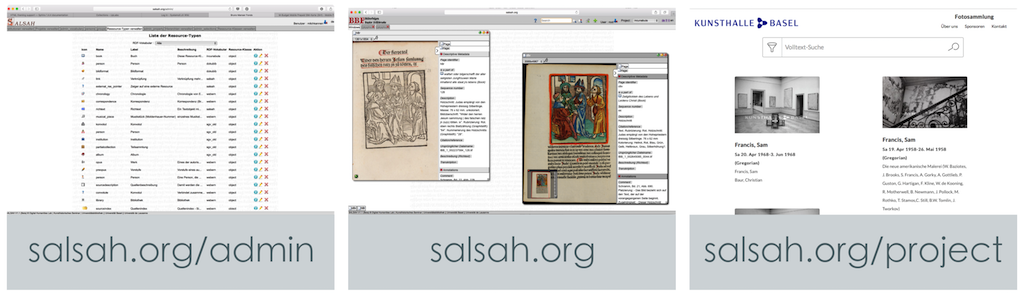
\includegraphics[width=\textwidth]{research-project-salsah1.png}
    \caption{SALSAH 1 with admin area (concept), work space (research) and project page (publication).}
\end{figure}

For SALSAH version 2 we're planning a different structure: The admin and the workspace interface would be on the same app route. The access to the admin area (projectSettings) depends on the user's rights. The project publication page can reuse the existing modules from SALSAH. But at the moment it's not clear how the URL structure will look like. ... http://dasch.org/[project]/[uuid] or http://project.knora.org/[uuid] 


The Data and Service Center for the Humanities (DaSCH) will use the SALSAH user interface. The DaSCH is implementing a distributed architecture with local or domain specific nodes which form a distributed peer-to-peer network. Resources can be made available to the other nodes at the discretion of each individual node. Authentication and user access is also organised in a distributed manner where each node has control whom it ``trusts''. In the near future, the Switch ``Swiss edu-ID'' will be used. For more information about Knora and the DaSCH: read the paper by Lukas Rosenthaler: Data and Service Center for the Humanities -- A National Service Architecture, July 2016.

%\begin{figure}[h]
%	\centering
%	\includegraphics[width=\textwidth]{DaSCHArchitectureLayout.jpg}
%	\caption{DaSCH's distributed architecture idea.  }
%\end{figure}

%\begin{itemize}
%	\item \textbf{http://salsah.org}\\The landing page for SALSAH with short information about the system and its connection to KnORA\footnote{KnORA stands for Knowledge Organization, Representation, and Annotation and builds the SALSAH backend: a RESTful API.} and the DaSCH\footnote{The Data and Service Center for the Humanities will use KnORA and SALSAH.}. A dominant login button brings the user to the SALSAH app.
%	\item \textbf{https://app.salsah.org}\\The app starts with a login screen and has the usual functions (reset password, registration?). After the login the user reaches the personal SALSAH workspace (\textbf{https://app.salsah.org/[username]}). With administration rights on a project, the user can define the project-specific resources, its properties and he can form the team right in this place. The admin area doesn't need an extra URL.
%	\item \textbf{http://docu.salsah.org}\\The SALSAH (and KnORA) documentation page based on the KnORA RST (reStructuredText) documents. The user has a direct link to that page from salsah.org and from app.salsah.org.
%	\item \textbf{https://page.salsah.org/[projectname]}\\ \textit{Here I'm not sure with the URL naming.}
%\end{itemize}

%We have also to think about the distributed network. Every university can have their own KnORA environment with the own SALSAH app. The notes above are just an example for the main installation in Basel.

%% SALSAH Architecture section:

\newpage
\section{SALSAH architecture}
\subsection{salsahFramework}
The main SALSAH app component is the framework module which builds the default layout template with

\begin{itemize}
	\item salsahHeader (Fig. \ref{fig:header}) with
	\begin{itemize}
		\item project selection and settings menu
		\item search bar panel incl. simple and extended search
		\item import menu (add resources and create collections)
		\item documentation menu (link to the documentation and/or cheat sheet)
		\item user menu (profile setting, log out etc.)
	\end{itemize}
	\item salsahFacetedSearch on the left hand side
	\item salsahView as a main container for salsahSearchResults, the graph and resource viewer, dashboard etc. The salsahView would be the frame for the ng2 router-outlet.
	\item salsahFooter (?)
\end{itemize}

\begin{figure}[h]
    \centering
    \includegraphics[width=\textwidth]{salsahFramework.png}
    \caption{salsahFramework}
    \label{fig:framework}
\end{figure}

\begin{figure}[h]
    \centering
    \includegraphics[width=\textwidth]{salsahHeader.png}
    \caption{salsahHeader}
    \label{fig:header}
\end{figure}

\begin{figure}[h]
    \centering
    \includegraphics[width=\textwidth]{salsahHeader_projectMenu-userMenu.png}
    \caption{salsahHeader}
    \label{fig:header}
\end{figure}

% 
% \begin{lstlisting}[caption=app.component template]
% \end{lstlisting}

%
%The salsahHeader is a mdToolbar with three sections:

%\textbf{left}
%	\begin{itemize}
%		\item md-icon-button (\textbf{menu}) to toggle the salsahNavigation menu
%		\item logo of the current/active project
%	\end{itemize}
%\textbf{center}
%	\begin{itemize}
%		\item salsahSearch with simpleSearch input field and
%		\item md-icon-button (\textbf{filter}) for extendedSearch
%	\end{itemize}
%\textbf{right}
%	\begin{itemize}
%		\item md-icon-button (\textbf{add}) opens the salsahImport/salsahAdd modal box
%		\item md-icon-button (\textbf{exit}) to log out
%	\end{itemize}


\newpage

\subsection{salsahSearch}
\subsubsection{simpleSearch}
\begin{figure}[!h]
    \centering
    \includegraphics[width=0.84\textwidth]{salsahSearch_focus.png}
    \caption{salsahSearch: focus on simpleSearch input shows recent search queries and saved extended search templates}
\end{figure}
\begin{figure}[!h]
    \centering
    \includegraphics[width=0.84\textwidth]{salsahSearch_keyevent.png}
    \caption{salsahSearch: keyevent in simpleSearch input shows a suggest-as-you-type list (incl. collection suggestions)}
\end{figure}

\newpage
\subsubsection{extendedSearch}
The extended search could look like a filter setting page in an e-mail application.

\begin{figure}[!h]
    \centering
    \includegraphics[width=\textwidth]{salsahSearch_extended.png}
    \caption{salsahSearch: extended search box}
\end{figure}

\newpage
\subsubsection{facetedSearch}
\begin{figure}[!h]
    \centering
    \includegraphics[width=\textwidth]{salsahSearch_faceted.png}
    \caption{salsahSearch: faceted search box on the left hand side}
\end{figure}

\newpage
\subsection{salsahView}
\subsubsection{gridView (search results and collections)}
\begin{figure}[!h]
    \centering
    \includegraphics[width=0.9\textwidth]{salsahView_grid.png}
    \caption{salsahView: grid (inspired by the old light table and the LFI news)}
\end{figure}

\subsubsection{listView (search results)}
\begin{figure}[!h]
    \centering
    \includegraphics[width=0.9\textwidth]{salsahView_list.png}
    \caption{salsahView: list (inspired by Google's inbox}
\end{figure}

\newpage

\subsubsection{tableView (search results of one resource type)}
\begin{figure}[!h]
    \centering
    \includegraphics[width=0.9\textwidth]{salsahView_table.png}
    \caption{salsahView: table (inspired by Excel)}
\end{figure}

From the list view (grid, list or tableView) the user can select more than one resource (well known from e-mail applications). In that case, an additional header provides some tools to do something with the selected resources. If the user selects some resources which are from the same resource type, he can edit them by one click. A modal box shows the properties of the selected resources. It's the same process as Apple's iTunes has (s. Fig. \ref{fig:itunes}).

\begin{figure}[!h]
    \centering
    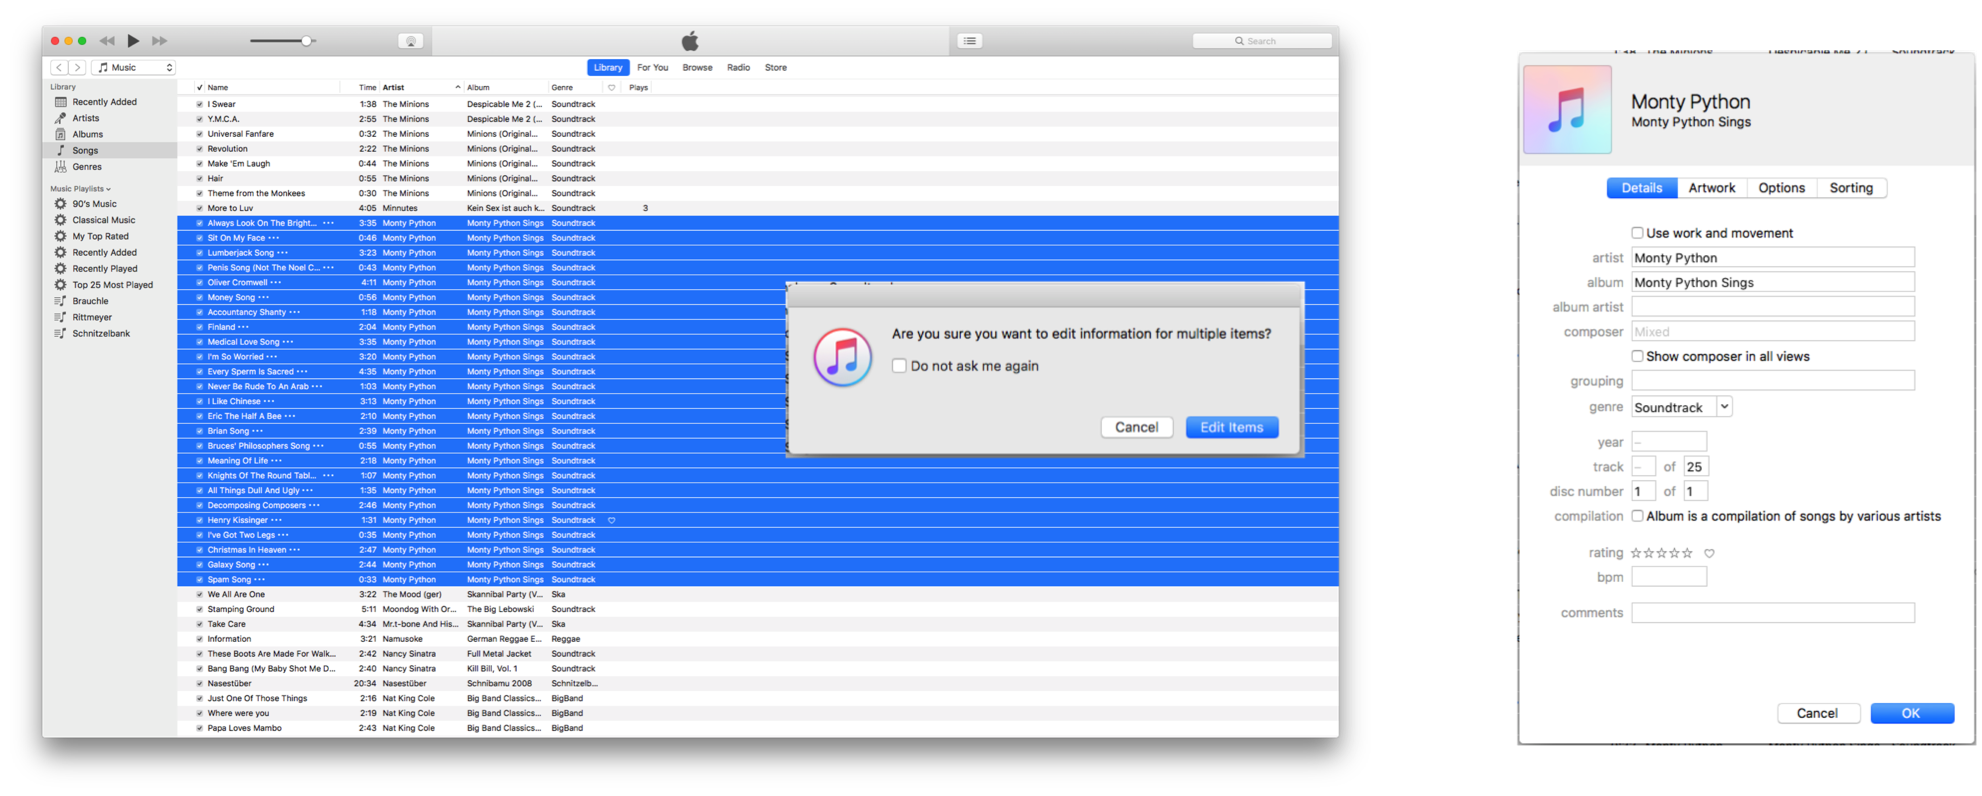
\includegraphics[width=0.9\textwidth]{iTunes-edit-selection.png}
    \caption{Example from iTunes: Selection of some songs; ``Get info'' opens a modal box, where the user can edit the properties for the whole selection.}
    \label{fig:itunes}
\end{figure}




\subsubsection{resourceView}
\begin{figure}[!h]
    \centering
    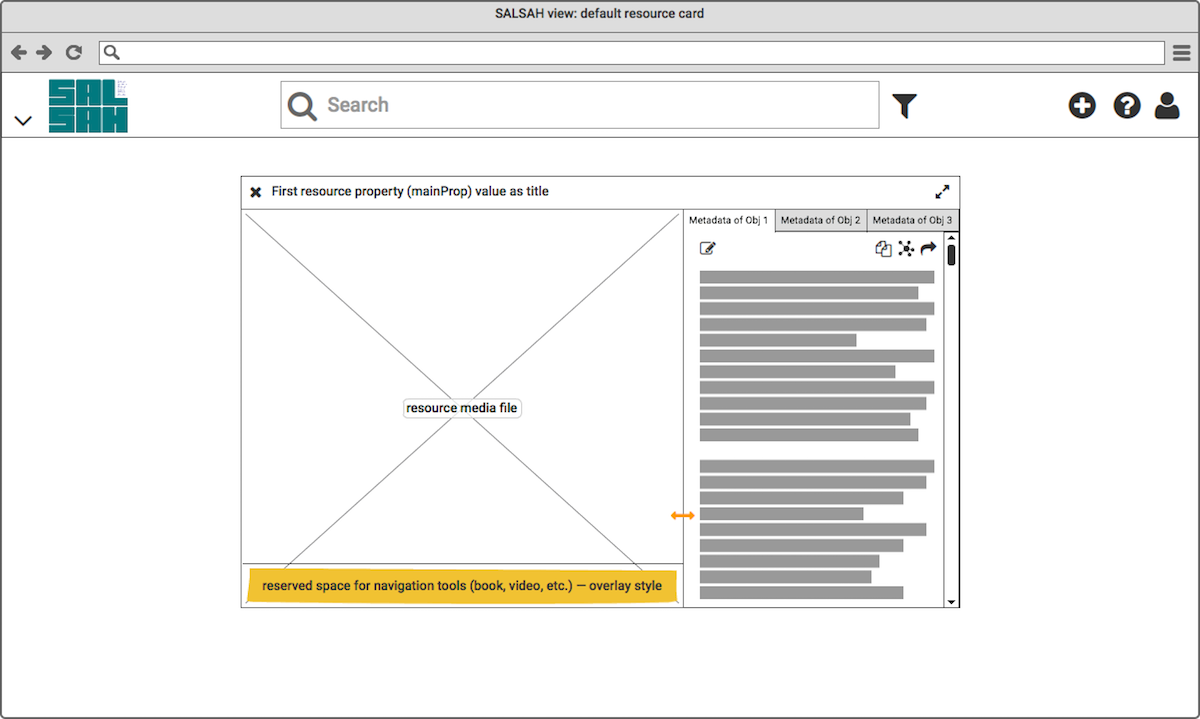
\includegraphics[width=0.9\textwidth]{salsahView_resource.png}
    \caption{salsahView: default resource card/modal (inspired by the window element of elementary OS)}
\end{figure}



\subsubsection{splitView (compare resources)}
Resource comparison viewer with a maximum of six flexible boxes.

\begin{figure}[!h]
    \centering
    \includegraphics[width=0.9\textwidth]{salsahView_split.png}
    \caption{salsahView: split (inspired by codepen.io)}
\end{figure}

\subsubsection{graphView}
Something with D3.js (d3js.org)

\subsubsection{dashboardView}
Place for activity thread includes updates from all projects the user is part of or has subscribed to. Activity thread should also be possible for user's activity.


\newpage
\subsection{salsahObject}

Like in SALSAH 1 we have a few predefined default resource objects. Most of the objects depend on the different kind of media types: emptyObject (object without a file, metadata only), imageObject, documentObject, videoObject, audioObject, collectionObject, regionObject, sequenceObject. Every salsah resource object needs his own viewer environment (card) with specific predefined tools.

\begin{itemize}
	\item \textbf{close} and \textbf{resize} the resource card; fullscreen and back to card size; (minimize? add the resource to one field (of 6) in the split view.)
	\item \textbf{change the view}: switch to the graph viewer or to the collection object, if the object is stored in a collection (link object).
	\item \textbf{share/add}: share the resource with friends or use the URI somewhere else (depends on the resource rights) / add the resource to a collection package (sth. like a playlist in music apps) -- we're using the collection also for links between at least two resources.
	\item \textbf{edit} (incl. delete) the resource (depends on the resource and property rights).
\end{itemize}


\subsubsection{emptyObject}
The empty object is an object without a media file; it has only metadata and the default tools as described above.

\subsubsection{imageObject}
The image object has additional tools like:
zoom, quality changer, rotate, mirror, transcriber, regions marker

\subsubsection{documentObject}
The document object is for pdf, latex or rtf, but also word etc. We're not able to display all the different document types -- in that case, we offer a download button.
The additional tools depending on the document viewer. But we need (+/-) zoom, quality changer, rotate, mirror, transcriber, regions marker.

\subsubsection{videoObject}
The moving image  needs some more tools:
timeline with preview, navigation (play, pause, stop, forward and rewind), scroll through, change quality, sequence marker (start/end), frame extraction, transcriber (incl. musical notation), transcription import (subtitle files e.g. srt)

Inspired by existing tools: Transcribe, f4, ELAN, MaxQData

\begin{figure}[!h]
    \centering
    \includegraphics[width=0.9\textwidth]{salsahObject_video.png}
    \caption{video Object (top left) embedded in the sequenceTranscription tool}
\end{figure}

\subsubsection{audioObject}

The audioObject could be similar to the videoObject. Perhaps we need an extra object for musical notes (musicNotationObject ?)


\subsubsection{collectionObject (collection / link / book) / salsahCollection}

\textbf{collectionObject/linkObject}

A collection connects various salsahObjects (resources). We can reuse the salsahCollection component for links and resource annotations as well. Every user should be able to create a collection and he can share it with others (share with the whole project team or with single user).


\textbf{bookObject}
The book is a special collectionObject with a navigation tool (sth. like timeline) incl. page preview and flick through. The single page includes the tools from the imageObject.



\subsubsection{regionObject (for images and documents)}


\subsubsection{sequenceObject (for video and audio)}



\newpage
\subsection{salsahProperty}
various GUI elements for different properties like salsahSelection (simple and hierarchical), salsahLocation (geonmame connection), salsahResourcePointer, salsahText, salsahNumber, salsahDate (simple and as a period), salsahTime, salsahRegion (?)

\subsubsection{stringElement (text)}


\subsubsection{numberElement (integer or floating point)}


\subsubsection{richtextElement (textarea)}


\subsubsection{dateElement (incl. period)}


\subsubsection{timeElement (incl. interval)}


\subsubsection{locationElement (connection to geonames.org)}


\subsubsection{resourcePointerElement (autocomplete or dropdown)}


\subsubsection{selectionElement (dropdown, checkbox or radio)}


\subsubsection{hierarchicalListElement (dropdown or radio)}


\subsection{salsahSettings}
\subsubsection{projectSettings}
Settings area for project admins. 

projectSettings includes:\\
projectProfile, projectMembers, projectVocabulary, projectProperties, projectSelections, projectHierarchicalLists, projectResources, projectSearchTemplates / projectFacetedSearch


\subsubsection{userSettings}
Settings area for the user's profile.


\newpage
\subsection{salsahExchange}
\subsubsection{importTools}
The SALSAH module ``importTools'' includes all kind of tools to add new objects into a project repository. They could be: createNewResource (single file upload \textit{(or addNewResource ?)}), addNewResources (multiple file upload\footnote{In SALSAH v1 we're using special PHP scripts to upload more than one file per time. These scripts are able to read csv-, filemaker- or other exported files. For SALSAH 2 it should be possible to have a feature like this in the front end. But at the moment it has a low priority status, because it's awkward to implement.}), but also createNewCollection, createNewLink and createNewProject (here we're not sure yet).

We're using the importTools with the top-level menu button ``add'' (+) -- selection menu -- and a modal box.


\subsubsection{exportTools}
Export a dataset as CSV...

\subsubsection{Some notes about the import (and export) process} % TITLE

\textbf{Three possible cases to transfer or to create data} % Major section

It's important to understand, at least to some degree, the subject or research of each project. This is necessary in order to translate (in the case of post mortem or in vivo) or create (ab ovo) an adequate data model to represent the data in the platform. The task of creating a data model requires considerable direct interaction with the researchers.

In the case of planned or starting projects (``ab ovo''), one difficulty is that researchers are not always familiar with the important concepts for their data models. Several examples (e.g. the Schweizerische Gesellschaft für Volkskunde, and the Anton Webern Edition) have shown that creating an adequate and efficient data model is essential for the success of a research project.

Already active projects (``in vivo'') often use tools and data models that are not optimal for the given task. Migration into the platform is often an opportunity to clean up the project's data models.

Post-mortem integration poses the biggest challenge. In one of the major test cases, the Lexicon Iconographicum Mythologiæ Classicæ, there is no documentation avail- able, and the people that created the data models and software are no longer available. However, there are still many active users who can help us to understand the concepts. Still, such projects require a great deal of time-consuming reverse engineering.

The two last cases (``in vivo'' and ``post mortem'') need special support from our side. Here we have to write an import script depending on the existing data. Perhaps it's possible to have an import button, where the user can upload the data exported from his previous database (Filemaker, MySQL, etc.).




\end{document}
